
\subsection{Judge Model Analysis}
\label{app:judge_model}
We analyze the judge model's performance on the labeled validation set. 
We compare \GraphEval{}'s judge model by using the last token logit as the judge model. This is a common practice in evaluating LLMs, as the last token logit is the most common way to extract the hidden state of the LLMs. We also analyze the judge model with or without the prompt encoder (PE), as it may have a negative impact on the judge model's performance. We refer to Figure~\ref{fig:evaluation_scores} for the judge model's performance on the labeled validation set. 


\begin{figure}[t]
\captionsetup[subfloat]{aboveskip=1pt,belowskip=1pt}
    \centering
    
\includegraphics[width=5.5in]{submissions/Jing2024/figures/experiments/evaluation_scores/legend_abla.pdf}\\
     \vspace{-5mm}
    \subfloat[LLaMA 7B]{
        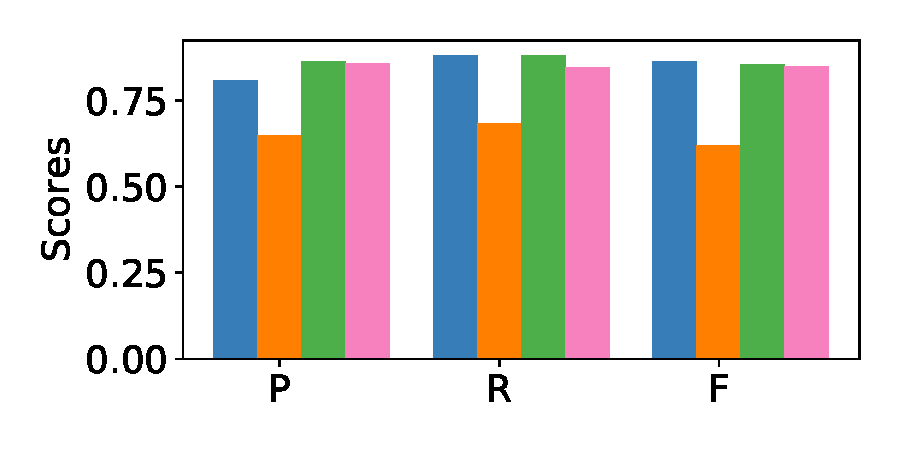
\includegraphics[width=1.78in]{submissions/Jing2024/figures/experiments/evaluation_scores/evaluation_scores_llama_2_7b.pdf}
        \label{fig:evaluation_scores_llama_2_7b}
       }\hspace{-4mm}
    \subfloat[LLaMA 13B]{
        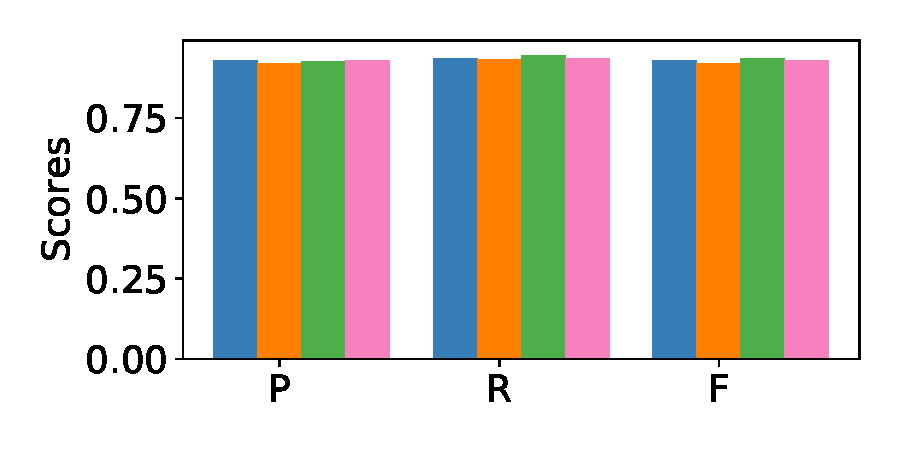
\includegraphics[width=1.78in]{submissions/Jing2024/figures/experiments/evaluation_scores/evaluation_scores_llama_2_13b.pdf}
        \label{fig:evaluation_scores_llama_2_13b}
       }\hspace{-4mm}
    \subfloat[LLaMA 70B]{
        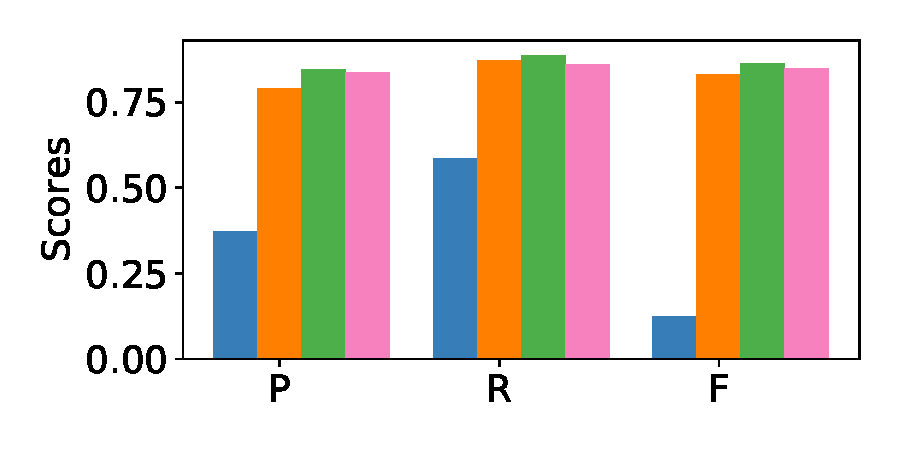
\includegraphics[width=1.78in]{submissions/Jing2024/figures/experiments/evaluation_scores/evaluation_scores_llama_2_70b.pdf}
        \label{fig:evaluation_scores_llama_2_70b}
       }
    \\\vspace{-4mm}
    \subfloat[Gemma 2B]{
        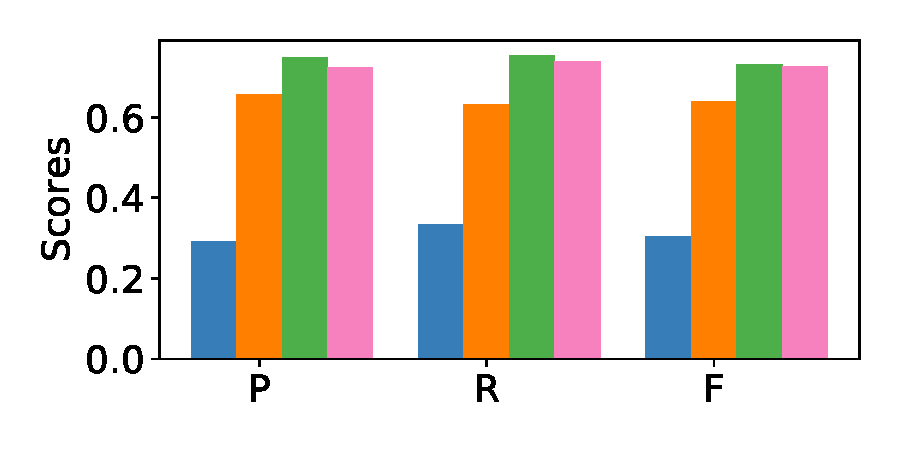
\includegraphics[width=1.78in]{submissions/Jing2024/figures/experiments/evaluation_scores/evaluation_scores_gemma_2b.pdf}
        \label{fig:evaluation_scores_gemma_2b}
       }\hspace{-4mm}
    \subfloat[Gemma 7B]{
        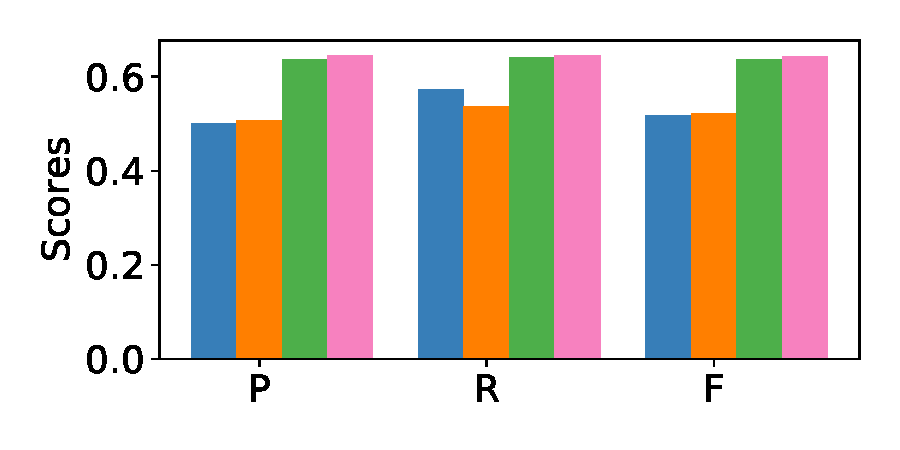
\includegraphics[width=1.78in]{submissions/Jing2024/figures/experiments/evaluation_scores/evaluation_scores_gemma_7b.pdf}
        \label{fig:evaluation_scores_gemma_7b}
       }\hspace{-4mm}
    \subfloat[Average]{
        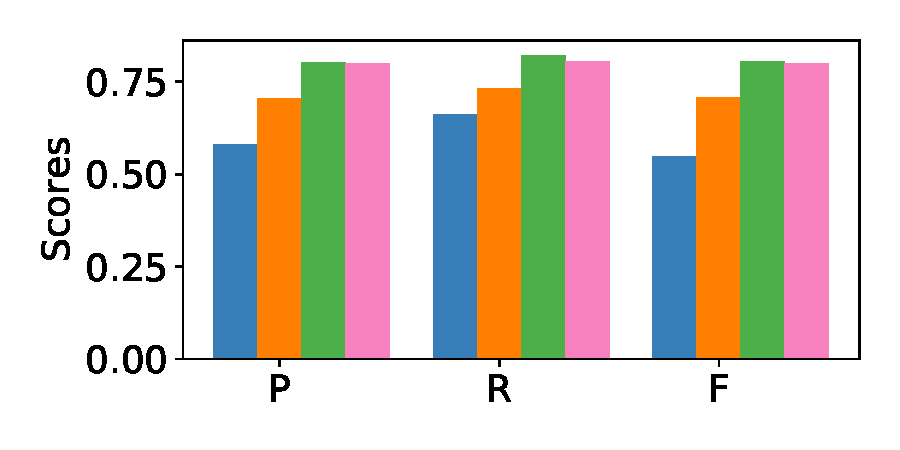
\includegraphics[width=1.78in]{submissions/Jing2024/figures/experiments/evaluation_scores/evaluation_scores_average.pdf}
        \label{fig:evaluation_scores_average}
       }
       \vspace{-3mm}
    \caption{Evaluation scores on the judge model's performance on the labeled validation set. P, R, and F are Precision, Recall, and F1 Score. 
    }
    \vspace{-3mm}
    \label{fig:evaluation_scores}
\end{figure}


\begin{table}[t]
    \centering
    \setlength{\tabcolsep}{2mm}{
    \begin{tabular}{lcccccccccc}
    \toprule
    \multirow{2}{*}{\textbf{Substitute Model}}  & \multicolumn{3}{c}{\textbf{LLaMA 2 7B}} & \multicolumn{3}{c}{\textbf{LLaMA 2 13B}} & \multicolumn{3}{c}{\textbf{LLaMA 2 70B}} \\
    \cmidrule(lr){2-4} \cmidrule(lr){5-7} \cmidrule(lr){8-10} 
    
    & P & R & F & P & R & F & P & R & F  \\
    \midrule
    \textbf{LLaMA 2 7B} & .858 & .845 & .850 & .928 & .934 & .930 & .837 & .861 & .848 \\
    \textbf{LLaMA 2 13B} & .850 & .868 & .855 & .930 & .940 & .932 & .837 & .851 & .844 \\
    \textbf{LLaMA 2 70B} & .868 & .883 & .871 & .924 & .942 & .931 & .858 & .876 & .866 \\
 
    \bottomrule
    \end{tabular}}
    \caption{Ablation on the LLaMA models as substitute models. The $i$-th row and $j$-th column denote the result of using $i$-th LLM as the substitute hidden state input for training on $j$-th model's labels.  P, R, and F are Precision, Recall, and F1 Score.  
    }
    \label{tab:abla_substitute}
    \end{table}


    






\begin{table}[t]
    \centering
    \small
    \setlength{\tabcolsep}{.5mm}{
    \begin{tabular}{lcccccccccc}
    \toprule
    \multirow{2}{*}{\textbf{Models}}
    & \multicolumn{2}{c}{\textbf{LLaMA 2 7B}} & \multicolumn{2}{c}{\textbf{LLaMA 2 13B}} & \multicolumn{2}{c}{\textbf{LLaMA 2 70B}} & \multicolumn{2}{c}{\textbf{Gemma 2B}} & \multicolumn{2}{c}{\textbf{Gemma7B}} \\
    \cmidrule(lr){2-3} \cmidrule(lr){4-5} \cmidrule(lr){6-7} \cmidrule(lr){8-9} \cmidrule(lr){10-11}
      & Speed & \#GPUs   & Speed & \#GPUs  & Speed & \#GPUs & Speed & \#GPUs & Speed & \#GPUs \\
    \midrule
    TG (A6000) & 2.26 & 1 & 1.07 & 2 & 0.09 & 4 & 2.06 (1.82) & 1 & 2.18 (1.28) & 1 \\
    \GraphEval{} (A6000) & 121.34  & 1 & 120.10 & 1 & 117.90 & 1 & 388.61 & 1 & 389.04 & 1 \\
    \midrule
    TG (A100) &  2.80 & 1 & 1.48 & 1 & 0.21 & 2 & 2.47 & 1 & 2.42 & 1 \\
    \GraphEval{} (A100) &  210.59 & 1 & 213.05 & 1 & 210.30 & 1 & 731.98 & 1 & 735.62 & 1 \\
    \bottomrule
    \end{tabular}}
    \caption{Efficiency evaluation. Speed denotes the average number of triple facts on which a conclusion can be given in one second. \#GPUs denotes the least number of GPUs to run without OOM. TG denotes text generation. 
     The numbers in parentheses are the speed without Flash Attention 2.}
    \label{tab:speed_test}
\end{table}

    


 \paragraph{Accuracy Analysis}
 The  \GraphEval{} model, both with and without Prompt Encoder (PE), consistently outperforms the score of using Last token logits in almost all configurations and metrics. This indicates the effectiveness of the  \GraphEval{} approach in capturing the nuances of the evaluation task.

 \paragraph{Ablation Study}
{\it On Prompt Encoder:}
As Figure~\ref{fig:evaluation_scores} shows, 
the comparison between models with and without PE indicates a slight performance variation. For \GraphEval{}, the presence of PE does not significantly alter the performance, suggesting that our method of evaluating LLMs is robust to the inclusion or exclusion of PE.
For the Last token logits method, removing PE generally results in a perturbation in performance. However, the  \GraphEval{} approach's consistency suggests a potentially different or more advanced mechanism of evaluation that is less dependent on PE.
{\it On Substitute Models:}
We also evaluate the judge model's performance on different LLMs as hidden state input. 
We refer to Table \ref{tab:abla_substitute} for the judge model's performance on different LLMs as hidden state input. We can see that, generally, when larger models are applied for feeding the hidden states, there is a slight increase in the fitting accuracy of the judge model. However, there is no significant difference in the judge model's performance.



\paragraph{Efficiency study}
We also analyze the judge model's efficiency by measuring the time it takes to make a prediction on one triple.
The speed of text generation refers to the average rate at which the LLM completes generating a response consisting of one sentence derived from a triple. It's important to recognize that the pace of text generation can vary with different prompts because the LLM may produce responses of varying lengths. Therefore, for a more consistent measure of text generation speeds, it's advisable to consider the rate of token generation. Despite this, our evaluation framework, \GraphEval{}, does not depend on text generation and operates on a triple-based unit. Consequently, we continue to use the triple as the unit of measurement for time.
We use the same hardware and software environment for all the experiments. We compare the average speed of the judge model with text generation. We report the time it takes to make a prediction in Table \ref{tab:speed_test}. 
 The attention implementation and precision are the same for text generation and for the judge model's input model. 
 We can see that the judge model is significantly faster than text generation. This indicates that the judge model is efficient in evaluating the LLMs. Also, benefiting from the substitute model, our evaluation speed and GPU requirement does not grow with the LLM size, which is an advantage for evaluating large LLMs.
 We also observe that, paradoxically, the Gemma 2B model operates slower than the Gemma 7B model, despite its smaller size. This counterintuitive result could be attributed to the implementation of Flash Attention 2. To draw a fair comparison, we documented the text generation speed on A6000 GPUs excluding Flash Attention 2, which is indicated within parentheses. The comparative data reveals that Gemma 2B is faster than Gemma 7B when Flash Attention 2 is not utilized. Notwithstanding this, Gemma 2B demonstrates enhanced performance when Flash Attention 2 is active. Therefore, for the sake of consistency, we have decided to maintain the results acquired with Flash Attention 2.
